\message{ !name(implementation.tex)}
\message{ !name(implementation.tex) !offset(18) }


	\includegraphics[width=0.3\linewidth]{img/v1.png}
	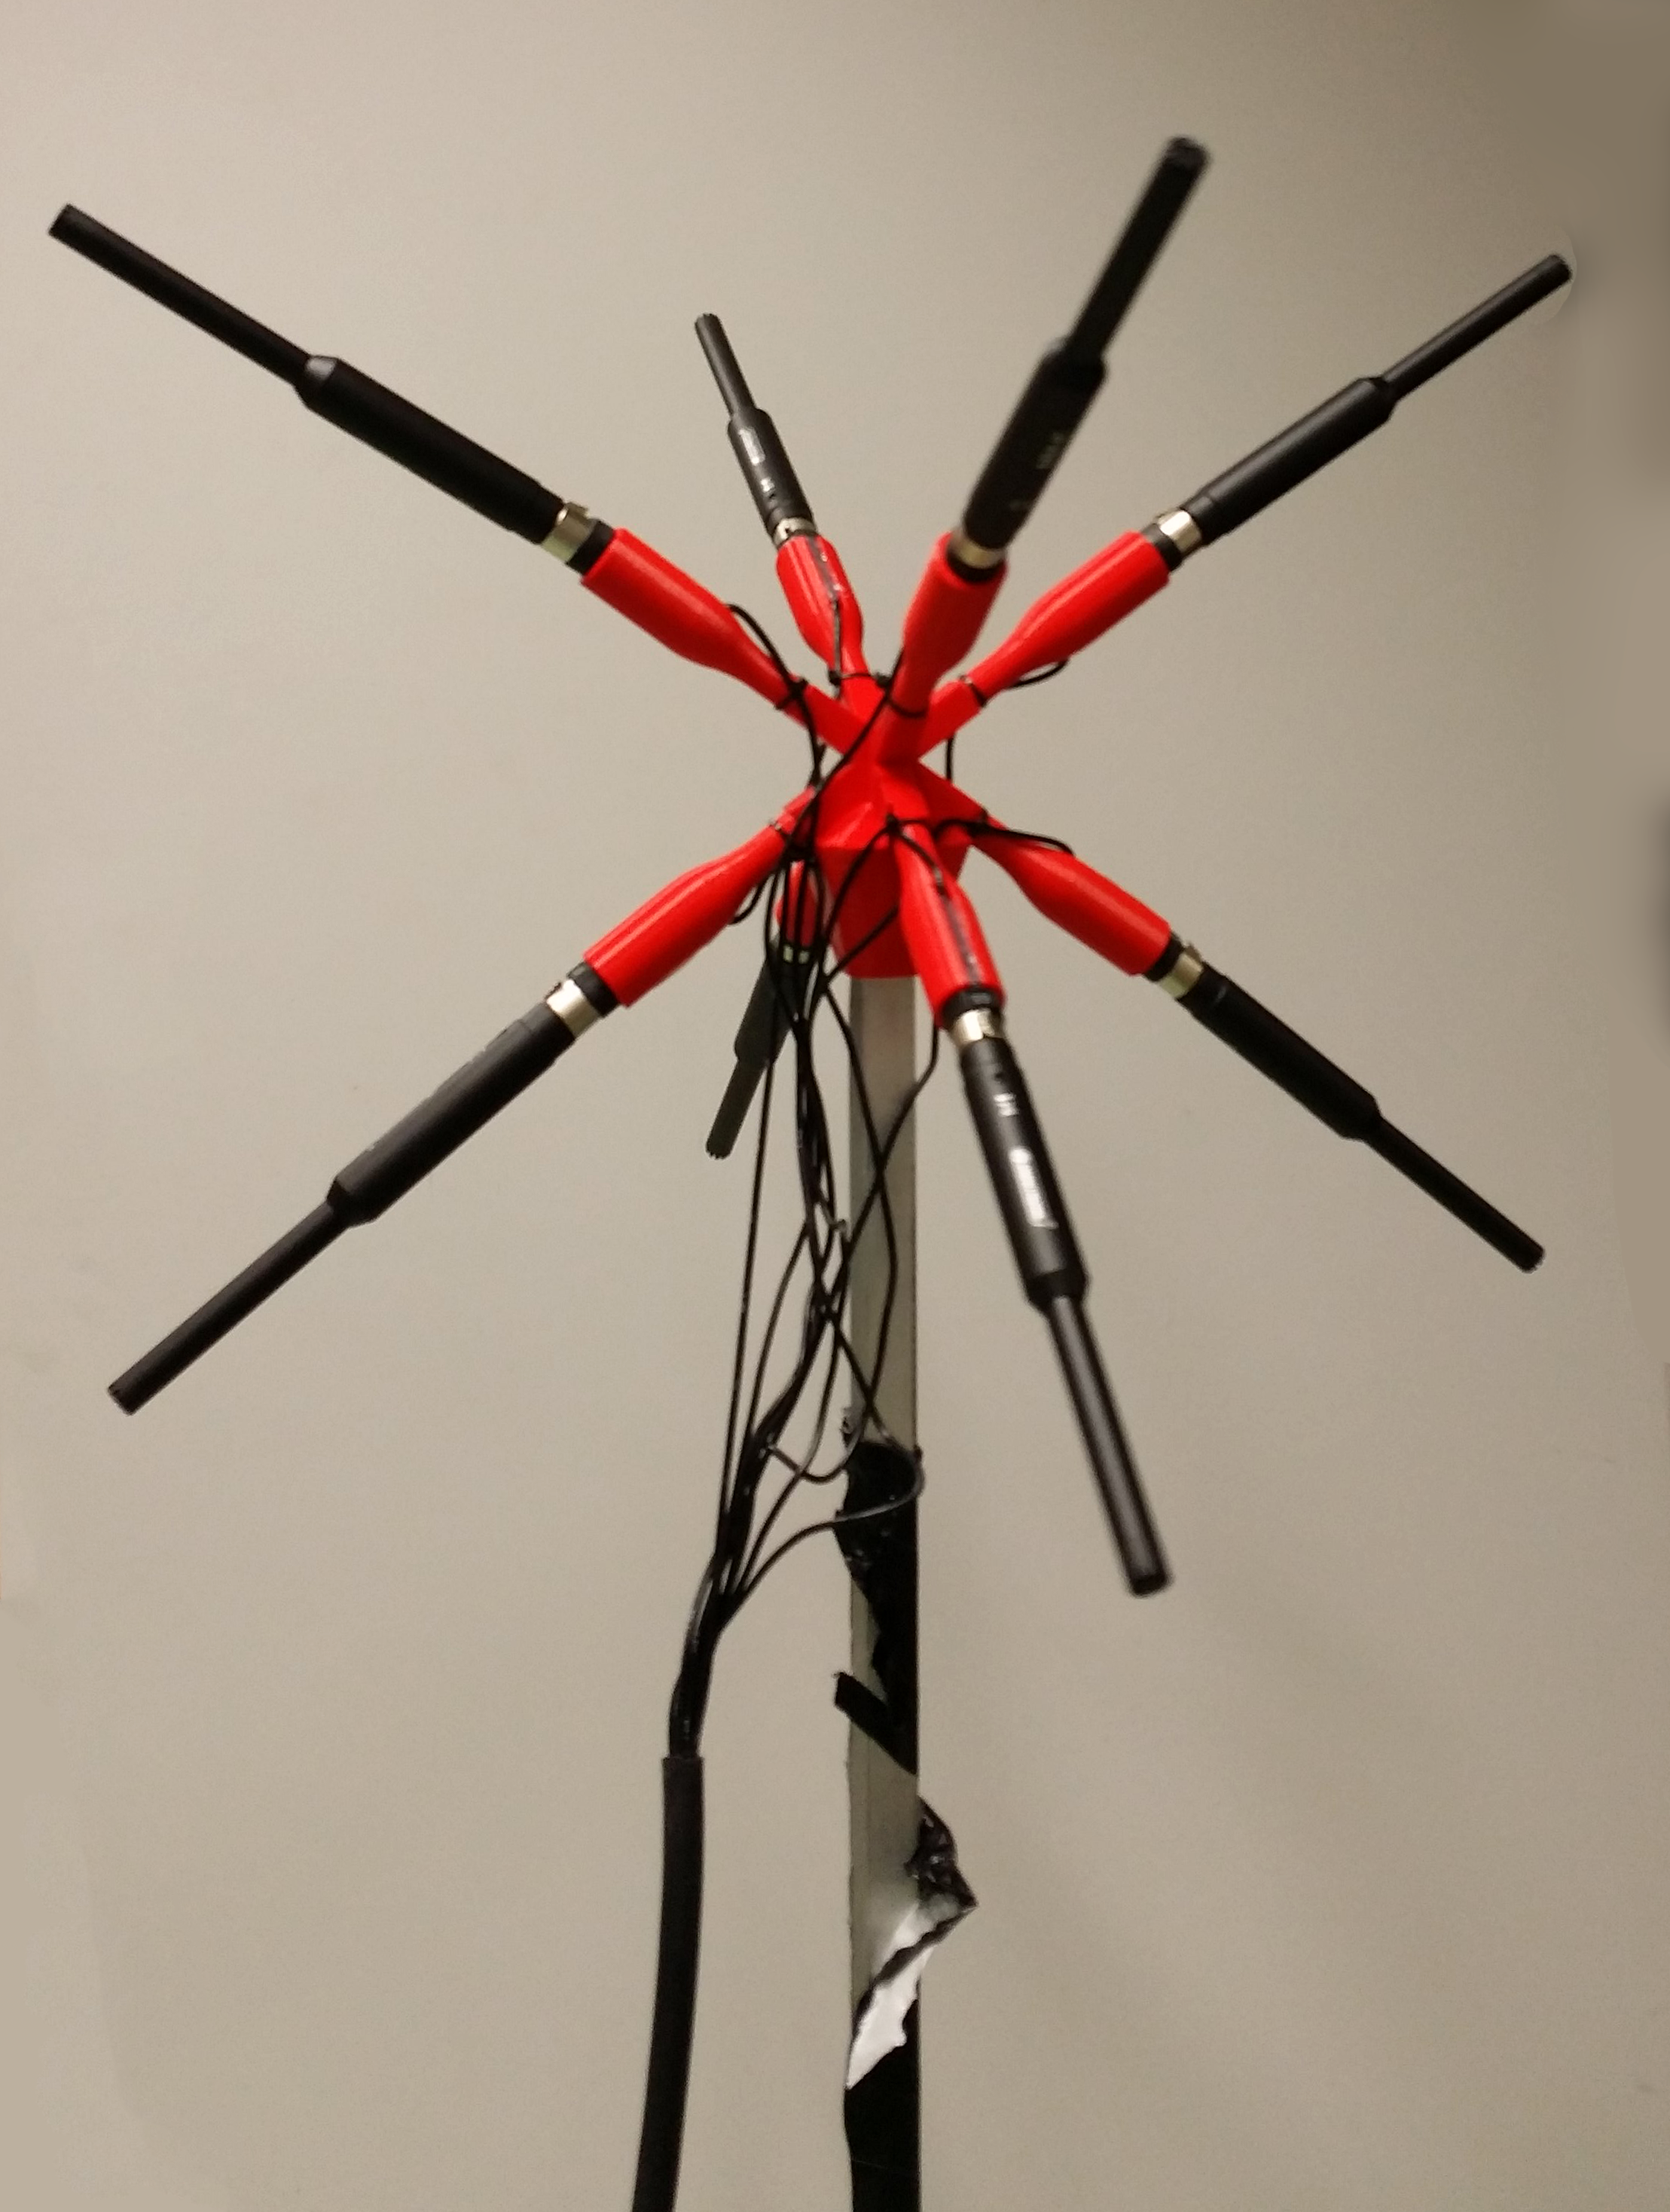
\includegraphics[width=0.3\linewidth]{img/v2.png}
	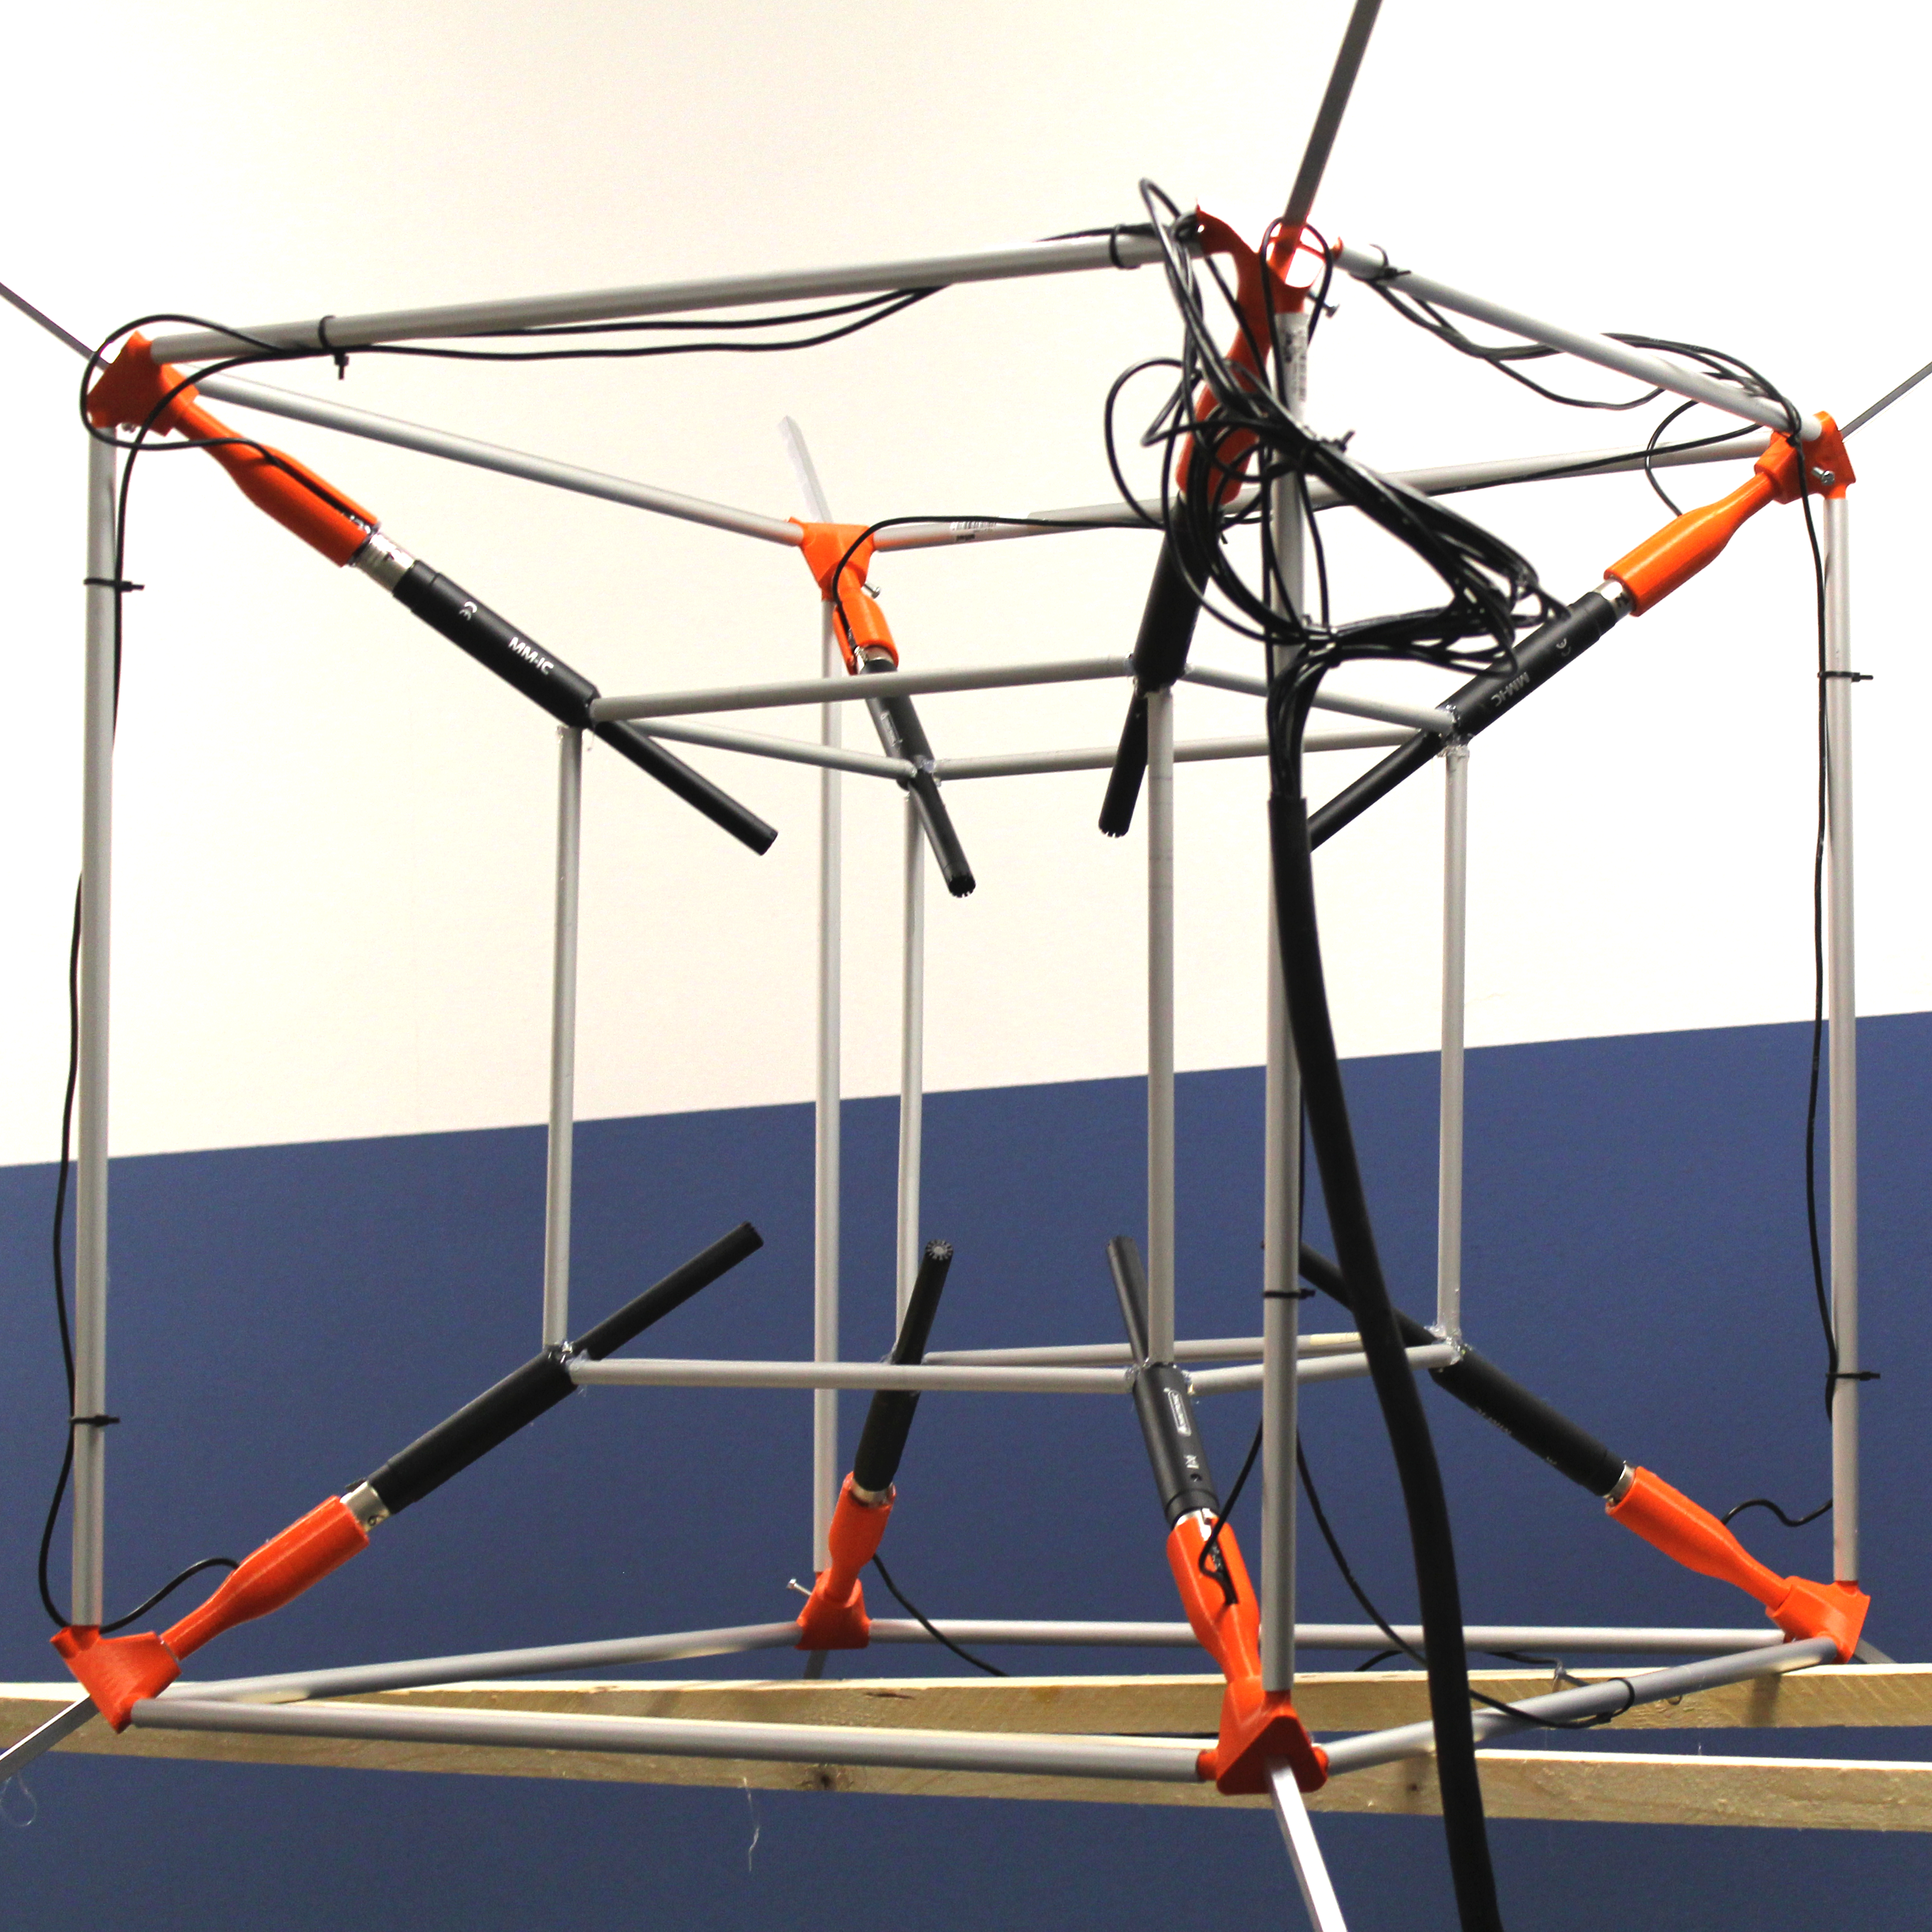
\includegraphics[width=0.3\linewidth]{img/v3.png}
	\caption{Aufbau unserer Messapparatur}
	\label{tet}
	%\vspace{-1cm}
\end{figure} \todo{add more \LaTeX skill}
Um das durch die Simulation evaluierbare Verfahren praktisch zu testen und zu nutzen, muss nur die Quelle der Daten, also das erste Modul, ausgetauscht werden. Die Aufgabe des ersten Moduls ist es nun nicht mehr, virtuelle Mikrofone  zu simulieren, die virtuelle Schallquellen aufnehmen. Stattdessen müssen die Signale echter Mikrofone, welche echte Schallquellen aufnehmen eingelesen werden. Um die Signale der Mikrofone mit einem Computer zu verarbeiten, müssen sie digitalisiert werden. Zusätzlich benötigt man eine alternative Implementation des ersten Moduls, die die Daten von der Hardware annimmt und an das zweite Modul weiterleitet. Hierbei kommen wieder die Vorteile unserer modularen Vorgehensweise zum Tragen, da nur das erste Modul ersetzt werden muss und die gesamte restliche Software beibehalten werden kann. Dies sorgt auch dafür, dass die Simulation und die Realwelttests immer die gleichen Auswertungsalgorithmen verwenden und so sehr gut vergleichbar sind.
\subsubsection{Mikrofonarray}
Die erste Komponente, die es bei einem realen Aufbau der Messapparatur eine wichtige Rolle spielt, ist die der Schallwandlung. Dies wird durch Mikrofone realisiert, an die es einige Anforderungen gibt. Die wichtigste Anforderung ist, dass sie eine möglichst kugelförmige Charakteristik haben.
Außerdem erzeugen kleine Mikrofone weniger Schallschatten und Reflexionen. Des Weiteren sollte das Signal-Rausch-Verhältnis möglichst groß sein, da Rauschen die Messungen unpräziser macht \cite{Rausch}.

Wir haben drei Prototypen unseres Mikrofonarrays konstruiert und diese dabei Optimiert. Der erste Prototyp unseres Mikrofonarrays bestand aus 4 Mikrofonen, die in einem Tetraeder angeordnet sind, da dies das absolute Minimum für eine dreidimensionale Richtungsbestimmung ist. Für diesen haben wir Elektretmikrofonkapseln verwendet, da diese Klein sind und verhältnismäßig gute Signalqualtität bieten, und teilweise eine Kugelcharakteristik besitzen.
Diese sollte möglichst gleichmäßig sein, da nur so aus allen Richtungen Töne mit gleicher Qualität aufgenommen werden können. Wenn zum Beispiel alle Mikrofone eine Nierencharakteristik aufweisen und sie in einem gleichseitigen Dreieck angeordnet sind, liefert mindestens ein Mikrofon ein deutlich schwächeres Signal als die anderen, was dazu führt, das die Phasenlage der einzelnen Wellen ungenauer bestimmt werden, und mit ihnen auch die Richtungsbestimmung ungenauer wird.
Um unter diesem Aspekt geeignete Elektretmikrofonkapseln zu finden, haben wir die Charakteristiken verschiedener Mikrofone mittels einer selbst entwickelten Messapparatur und einer selbst entwickelten Messsoftware vermessen. Die hierfür entwickelte Messapparatur sendet mittels eines Lautsprechers eine Sinus-Schwingung aus und misst, wie stark diese vom Mikrofon aufgenommen wurde. Danach dreht sie das Mikrofon um einen festgelegten Winkel weiter und fertigt erneut eine Messung an. Dieser Vorgang wird solange wiederholt, bis das Mikrofon einmal um 360$^{\circ}$ gedreht wurde.
\begin{figure}[H]
  \centering
  \includegraphics[width=0.8\linewidth]{img/chara_mess}
  \caption{Unsere Messapparatur für die Charakteristik eines Mikrofons}
\end{figure}
\todo{messapperatur raus?}
Die so ermittelten Daten können nun mittels des freien Plottingprogramms \textit{gnuplot}~\cite{Gnuplot} visualisiert werden, um die Richtcharakteristik abzulesen.
\begin{figure}[H]
  \centering
  \includegraphics[width=0.45\linewidth]{img/badMic}
  \includegraphics[width=0.45\linewidth]{img/goodMic}
  \caption{Auf den beiden Grafiken ist die gemessene Amplitude des Mikrofons über den Winkel aufgetragen. Bei der linken Grafik kanmn an feststellen, dass das vermessene Mikrofon eine sehr ungleichmäßige Charakteristik aufweist, diese Mikrofone haben wir zu Anfang verwendet. Auf der rechten Seite ist die Charakteristik der Mikrofone zu sehen, die wir in unserem aktuellen Testaufbau verwenden. Diese ist sehr gleichmäßig, weshalb wir diese Mikrofone verwendet haben.}\label{fig:caracter}
\end{figure}
Dadurch, dass unser Tetraeder symmetrisch ist, sind die Fehler in alle Richtungen ungefähr gleich groß und die Richtungsbestimmung ist in allen Richtungen gleich gut. Um die Charakteristik der Mikrofone möglichst wenig zu verändern, haben wir die Mikrofone nur an ihrem Kabel mit dem Tetraeder verbunden. Dadurch ist der Schallschatten durch den Tetraeder relativ gering. Das Mittelstück des Tetraeders haben wir mit Hilfe eines 3D-Druckers hergestellt (siehe Abbildung \ref{tet}).\\

Der zweite Optimierungsschritt des Mikrofonarrays beinhaltete eine Erhöhung der Mikrotonanzahl von 4 auf 8 und einen Umstieg auf eine würfelförmige Anordnung. Hierdurch stehen mehr Informationen für den Richtungsbestimmungsalgorithmus zur Verfügung und das Gleichungssystem wird überbestimmt. Auch sind wir von Elektretmikrofonkapseln auf Professionelle Messmikrofone umgestiegen, da diese eine Definierte Charakteristik haben und ein besseres Signal-Rausch Verhältnis aufweisen.

Da beim zweiten Prototyp des Mikrofonarrays die Mikrofone der Abstand zwischen den Mikrofonen sehr groß war und dadurch das nutzbare Frequenzspektrum nach oben hin sehr stark eingeschränkt wurde, war das Ziel des dritten Prototyps diese wieder näher aneinander zu rücken. Dieses Ziel erreichten wir durch eine Umkehrung der Mikrotonrichtung, so dass diese nun nicht mehr von innen nach außen, sondern von Außen nach innen zeigen.
\subsubsection{Audiointerface}
Auch für das Audiointerface, also die Verbindung zwischen Mikrofonen und Computer, gibt es bestimmte Voraussetzungen. So benötigt unser Verfahren mindestens 4 Mikrofone, jedoch lässt es sich einfach auf mehr Kanäle erweitern, was der Genauigkeit zugute kommt. Daher haben wir ein Audiointerface mit möglichst vielen Kanälen gesucht. Eine weitere wichtige Anforderung an das Audiointerface ist eine hohe Auflösung, da hierdurch die Signalqualität verbessert wird und digitale Verstärkung bei ausreichender Audioqualität möglich ist. Um die Elekretmikrofonkapseln an das Audiointerface anzuschließen, benötigt man zusätzlich eine Schaltung, welche das unsymmetrische Signal der Elektretmikrofonkapsel in ein symmetrisches Signal für das Audiointerface umwandelt. Außerdem muss diese die Phantomspeisung, die das Audiointerface bereitstellt und eine Spannung von 48V hat, in eine Tonaderspeisung für das Mikrofon konvertieren. Hierfür kommt die Schaltung von \cite{Powering_microphones} zum Einsatz.

\subsubsection{Software}
Um die echten Mikrofone für die Richtungsbestimmung zu verwenden, muss noch eine Verbindung zwischen dem Audiointerface und dem nächsten Modul geschaffen werden. Durch unseren modularen Aufbau lässt sich dies leicht implementieren. Wir haben dazu ein Programm in Java entwickelt, das fähig ist, mehrkanalige Audiosignale in Echtzeit aufzunehmen und über TCP/IP an die Fourier-Transformation weiterzuleiten. Zur Umsetzung haben wir die Programmbibliothek \textit{portaudio} \cite{portaudio} verwendet. Diese Programmbibliothek hat den Vorteil, dass mehrere Audiokanäle zeitsynchronisiert eingelesen werden können, was sehr wichtig ist, damit unser Verfahren zur Richtungsbestimmung, welches auf der relativen Phasenlage basiert, funktioniert. \textit{Portaudio} haben wir in Java über das Java Native Interface (JNI) benutzt.

\subsection{Fourier-Transformation (Modul 2)}
Dieses Modul teilt die Audio-Signale in einzelne Sinuswellen und bestimmt deren Phase und Amplitude. Um dies zu bewerkstelligen, lässt sich eine diskrete Fourier-Transformation verwenden. Die diskrete Fourier-Transformation bestimmt aus einem zeitdiskretem Signal die einzelnen Sinusschwingungen mit ihrer zugehörigen Phase und Amplitude, die zusammen das Signal bilden. Ein schneller Algorithmus, um die diskrete Fourier-Transformation eines Signals zu berechnen, ist die Fast Fourier-Transformation (FFT). Dieser ist schnell genug, um eine Echtzeitverarbeitung des Signals zu ermöglichen. Als Implementation der FFT haben wir \textit{FFTW}\cite{FFTW} verwendet, da \textit{FFTW} kostenlos, opensource und vergleichsweise schnell ist.
Das Fourier-Transformations-Modul wurde aus Performancegründen in \textit{C++} implementiert.
Durch eine diskrete Fourier-Transformation von $n$ reellen Zahlen erhält man eine Liste aus $n$ komplexen Zahlen. Eine komplexe Zahl $z$ an der Stelle $j$ enthält die Amplituden- und Phaseninformation für die Frequenz $f$:
$$
f = \frac{j\cdot r}{n}

\message{ !name(implementation.tex) !offset(-51) }
